\documentclass[10pt]{beamer}

\mode<presentation>{% Settings
    % link to view http://www.hartwork.org/beamer-theme-matrix/
    % ------------------------------------------------------------------------------
    % Slide Themes
    % ------------------------------------------------------------------------------
    %\usetheme{default}
    %\usetheme{AnnArbor}
    %\usetheme{Antibes}
    %\usetheme{Bergen}
    \usetheme{Berkeley}
    %\usetheme{Berlin}
    %\usetheme{Boadilla}
    %\usetheme{CambridgeUS}
    %\usetheme{Copenhagen}
    %\usetheme{Darmstadt}
    %\usetheme{Dresden}
    %\usetheme{Frankfurt}
    %\usetheme{Goettingen}
    %\usetheme{Hannover}
    %\usetheme{Ilmenau}
    %\usetheme{JuanLesPins} % rounded title, gradient at top with section, no bottom bar
    %\usetheme{Luebeck}     % square title, toc at top of each slide
    %\usetheme{Madrid}      % rounded title
    %\usetheme{Malmoe}
    %\usetheme{Marburg}
    %\usetheme{Montpellier}
    %\usetheme{PaloAlto}
    %\usetheme{Pittsburgh}
    %\usetheme{Rochester}
    %\usetheme{Singapore}
    %\usetheme{Szeged}
    %\usetheme{Warsaw}

    % ------------------------------------------------------------------------------
    % Color Schemes
    % ------------------------------------------------------------------------------
    %\usecolortheme{default}
    %\usecolortheme{albatross}  % blue background with darker blue
    %\usecolortheme{beaver}     % gray with red
    %\usecolortheme{beetle}     % gray background
    %\usecolortheme{crane}      % orange
    \usecolortheme{dolphin}     % white with purple
    %\usecolortheme{dove}       % all white
    %\usecolortheme{fly}        % all gray including background
    %\usecolortheme{lily}       % white with blue
    %\usecolortheme{orchid}     % default blue
    %\usecolortheme{rose}       % default blue
    %\usecolortheme{seagull}    % darker gray than seahorse
    %\usecolortheme{seahorse}   % light gray blueish tint
    %\usecolortheme{whale}      % default blue
    %\usecolortheme{wolverine}  % yellow with a little blue

    %\setbeamertemplate{footline} % To remove the footer line in all slides uncomment this line
    %\setbeamertemplate{footline}[page number] % To replace the footer line in all slides with a simple slide count uncomment this line
    \setbeamertemplate{navigation symbols}{} % To remove the navigation symbols from the bottom of all slides uncomment this line
    \setbeamertemplate{bibliography item}{\insertbiblabel} % to number bibliography entries
}

\usepackage{Logemann}
\usepackage{Integral}
\usepackage{LinearAlgebra}
\usepackage{Derivative}
\usepackage{Vector}
\usepackage{Sum}
\usepackage{SetTheory}
\usepackage{booktabs}
\usepackage[backend=biber]{biblatex}
\addbibresource{refs.bib}

\title[]{Discontinuous Galerkin Method for Solving Thin Film Equations} % The short title
% appears at the bottom of every slide, the full title is only on the title page

\author{Caleb Logemann \and James Rossmanith} % Your name
\institute[Iowa State University]{% Your institution as it will appear on the bottom of every slide, may be shorthand to save space
Mathematics Department,\\ Iowa State University \\ % Your institution for the title page
\medskip
\textit{logemann@iastate.edu}} % Your email address

\date{May 13, 2019} % Date, can be changed to a custom date

\begin{document}
  \begin{frame}
    \titlepage{}
  \end{frame}

  \begin{frame}
    \frametitle{Overview}
    \tableofcontents
  \end{frame}

  \section{Thin Film Equation}
    \subsection{Model}
      \begin{frame}
        \frametitle{Model Equations}
        \begin{center}
          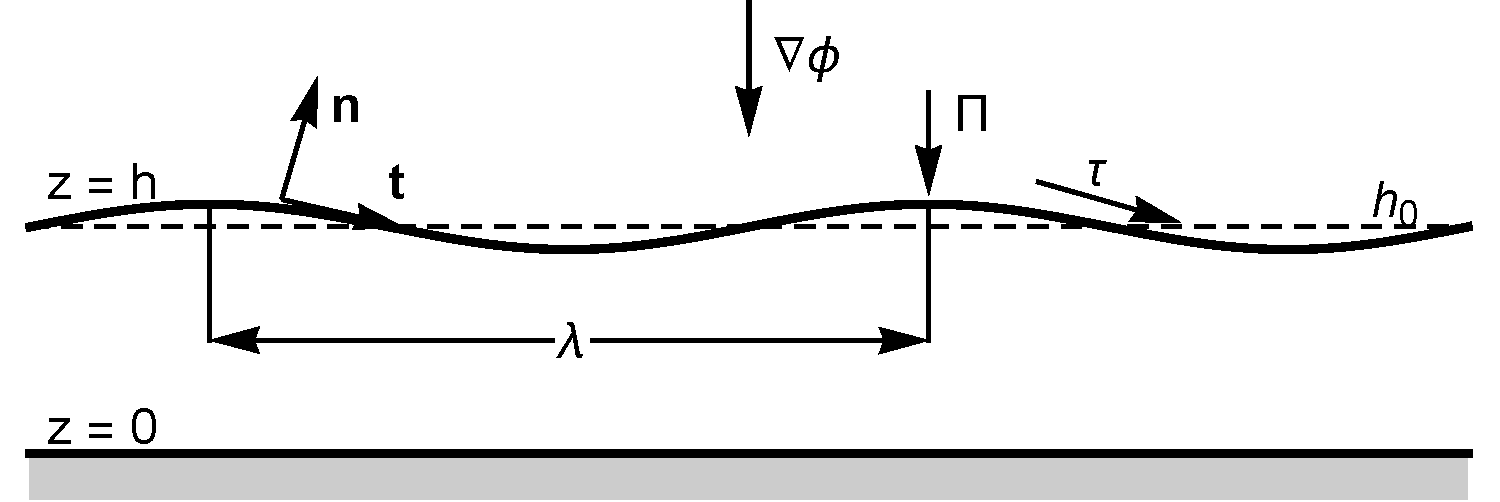
\includegraphics[scale=0.35]{Figures/ThinFilm.pdf}
        \end{center}
        \begin{itemize}
          \item Incompressible Navier-Stokes Equation
            \begin{align*}
              u_x + w_z &= 0 \\
              \rho\p{u_t + u u_x + w u_z} &= -p_x + \mu \Delta u - \phi_x \\
              \rho\p{w_t + u w_x + w w_z} &= -p_z + \mu \Delta w - \phi_z \\
              w &= 0, u = 0 &\text{at } z = 0 \\
              w &= h_t + u h_x &\text{at } z = h\\
              \v{T} \cdot \v{n} &= \p{-\kappa \sigma + \Pi}\v{n} + \p{\pd{\sigma}{s} + \tau}\v{t} &\text{at } z = h
            \end{align*}
        \end{itemize}
      \end{frame}

      \begin{frame}
        \begin{center}
          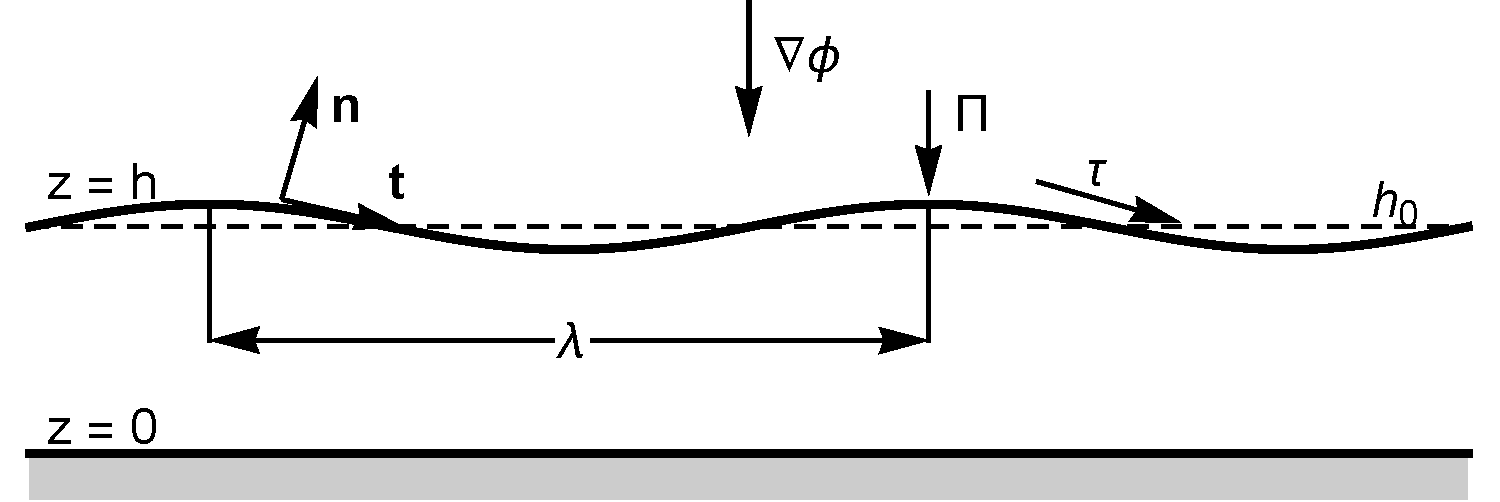
\includegraphics[scale=0.35]{Figures/ThinFilm.pdf}
        \end{center}
        Nondimensionalize, integrate over \(Z\), and simplify, gives

        \small{\begin{gather*}
          H_T + \p{\frac{1}{2}\p{\tau + \Sigma_X}H^2 - \frac{1}{3}\p{\eval{\Phi}{Z = H} - \Pi}_X H^3}_X = - \frac{1}{3}\bar{C}^{-1}\p{H^3 H_{XXX}}_X
        \end{gather*}}

        \begin{gather*}
          q_t + \p{q^2 - q^3}_x = - \p{q^3 q_{xxx}}_x
        \end{gather*}
      \end{frame}
    \subsection{Numerical Methods}
      % IMEX
      % Convection DG
      % LDG
      % Picard Iteration
      \begin{frame}
        \begin{itemize}
          \frametitle{Method Overview}
          \item Simplified Model
            \[
              q_t + \p{q^2 - q^3}_x = -\p{q^3 q_{xxx}}_x \qquad \p{0, T} \times \Omega
            \]

          \item Runge Kutta Implicit Explicit (IMEX)
            \begin{align*}
              q_t &= F(q) + G(q)
            \end{align*}
            \begin{itemize}
              \item F evaluated explicitly
              \item G solved implicitly
            \end{itemize}
            \begin{align*}
              F(q) &= -\p{q^2 - q^3}_x  \\
              G(q) &= \p{q^3 q_{xxx}}_x
            \end{align*}

        \end{itemize}
      \end{frame}

      \begin{frame}
        \frametitle{Convection}
        \begin{itemize}
          \item Convection Equation
            \begin{gather*}
              F(q) = f\p{q}_x = 0 \qquad \p{0, T} \times \Omega \\
              f(q) = q^2 - q^3
            \end{gather*}

          \item Weak Form \hfill \\
            Find \(q\) such that
            \[
              \dintt*{\Omega}{}{F(q) v - f(q) v_x}{x} + \eval{\hat{f}v}{\partial\Omega} = 0
            \]
            for all test functions \(v\)
        \end{itemize}
      \end{frame}

      \begin{frame}
        \frametitle{Notation}
        \begin{itemize}
          \item Partition the domain, \(\br{a, b}\) as
            \[
              a = x_{1/2} < \cdots < x_{j-1/2} < x_{j+1/2} < \cdots < x_{N + 1/2} = b
            \]

          \item \(I_j = \br{x_{j-1/2}, x_{j+1/2}}\)
          \item \(x_j = \frac{x_{j+1/2} + x_{j-1/2}}{2}\).
            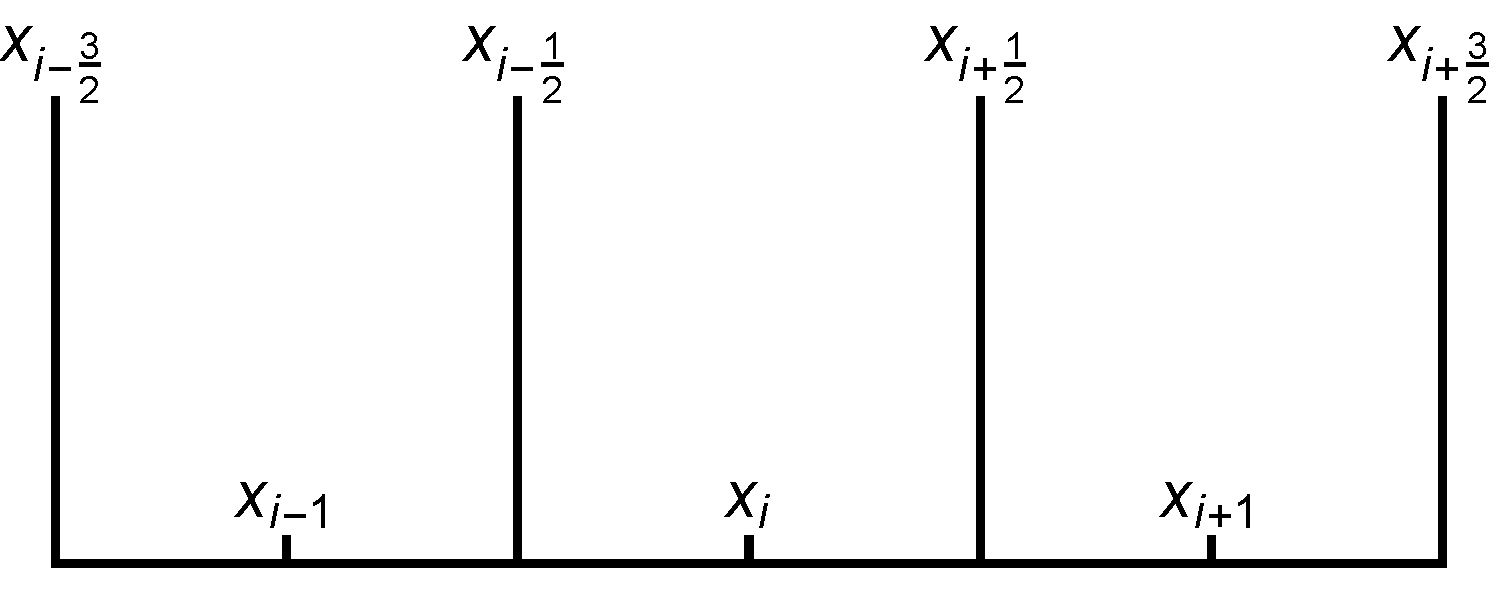
\includegraphics[scale=0.35]{Figures/Cells.pdf}
        \end{itemize}
      \end{frame}

      \begin{frame}
        \frametitle{Runge Kutta Discontinuous Galerkin}
        \begin{itemize}
          \item
            Find \(Q(t,x)\) such that for each time \(t \in \p{0, T}\), \(Q(t, \cdot) \in V_h = \set{v \in L^1(\Omega): \eval{v}{I_j} \in P^k(I_j)}\)
            \begin{align*}
              \dintt{I_j}{}{F(Q) v}{x} &= \dintt{I_j}{}{f(Q)v_x}{x} \\
              &- \p{\mcF_{j + 1/2}v^-(x_{j+1/2}) - \mcF_{j - 1/2}v^+(x_{j-1/2})}
            \end{align*}
            for all \(v \in V_h\)

          \item Rusanov/Local Lax-Friedrichs Numerical Flux
            \small{\[
              \mcF_{j+1/2} = \frac{1}{2}\p{f\p{Q^-_{j+1/2}} + f\p{Q^+_{j+1/2}}} + \frac{1}{2}\max[q]{\abs{f'(q)}}\p{Q^-_{j+1/2} - Q^+_{j+1/2}}
            \]}
        \end{itemize}
      \end{frame}

      \begin{frame}
        \frametitle{Diffusion}
        \begin{itemize}
          \item Diffusion Equation
            \begin{align*}
              G(q) &= -\p{q^3 q_{xxx}}_x \qquad \p{0, T} \times \Omega
            \end{align*}

          \item Local Discontinuous Galerkin
            \begin{align*}
              r &= q_x \\
              s &= r_x \\
              u &= s_x \\
              G(q) &= \p{q^3 u}_x
            \end{align*}
        \end{itemize}
      \end{frame}

      \begin{frame}
        \frametitle{Local Discontinuous Galerkin}
        Find \(Q(t, x), R(x), S(x), U(x)\) such that for all \(t \in \p{0, T}\)
        \(Q(t, \cdot), R, S, U \in V_h = \set{v \in L^1(\Omega): \eval{v}{I_j} \in P^k(I_j)}\)
        \begin{align*}
          \dintt{I_j}{}{R v}{x} &= -\dintt{I_j}{}{Q v_x}{x} + \p{\hat{Q}_{j+1/2}v^-_{j+1/2} - \hat{Q}_{j-1/2} v^+_{j-1/2}} \\
          \dintt{I_j}{}{S w}{x} &= -\dintt{I_j}{}{R w_x}{x} + \p{\hat{R}_{j+1/2}w^-_{j+1/2} - \hat{R}_{j-1/2} w^+_{j-1/2}} \\
          \dintt{I_j}{}{U y}{x} &= -\dintt{I_j}{}{S y_x}{x} + \p{\hat{S}_{j+1/2}y^-_{j+1/2} - \hat{S}_{j-1/2} y^+_{j-1/2}} \\
          \dintt{I_j}{}{G(Q) z}{x} &= -\dintt{I_j}{}{Q^3 U z_x}{x} + \p{\hat{U}_{j+1/2}z^-_{j+1/2} - \hat{U}_{j-1/2} z^+_{j-1/2}}
        \end{align*}
        for all \(I_j \in \Omega \) and all \(v, w, y, z \in V_h\).
      \end{frame}

      \begin{frame}
        \frametitle{Numerical Fluxes}
        \begin{align*}
          \hat{Q}_{j+1/2} &= Q^+_{j+1/2} \\
          \hat{R}_{j+1/2} &= R^-_{j+1/2} \\
          \hat{S}_{j+1/2} &= S^+_{j+1/2} \\
          \hat{U}_{j+1/2} &= \p{Q^3 U}^-_{j+1/2}
        \end{align*}
        \begin{center}
          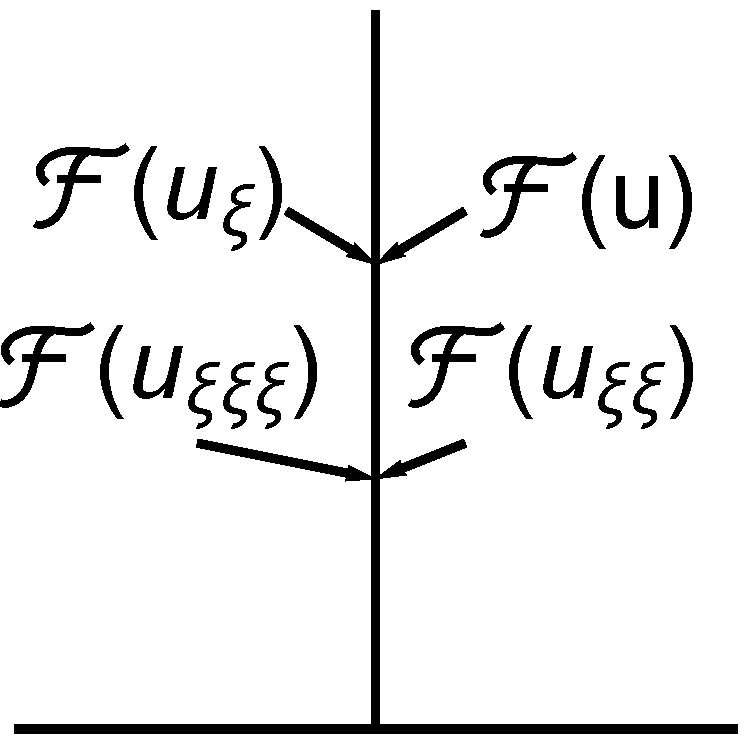
\includegraphics[scale=0.3]{Figures/localDG.pdf}
        \end{center}
      \end{frame}

      \begin{frame}
        \frametitle{IMEX Runge Kutta}
        \begin{itemize}
          \item IMEX scheme
            \begin{align*}
              q^{n+1} &= q^n + \Delta t \sum{i = 1}{s}{b_i' F(t_i, u_i)} + \Delta t \sum{i=1}{s}{b_i G(t_i, u_i)} \\
              u_i &= q^n + \Delta t \sum{j = 1}{i-1}{a_{ij}' F(t_j, u_j)} + \Delta t \sum{j=1}{i}{a_{ij} G(t_j, u_j)} \\
              t_i &= t^n + c_i \Delta t
            \end{align*}

          \item Double Butcher Tableaus \hfill \\ \hfill \\
            \begin{tabular}{r|l}
              \(c'\) & \(a'\) \\
              \midrule
                & \(b'^T\)
            \end{tabular}
            \begin{tabular}{r|l}
              \(c\) & \(a\) \\
              \midrule
                & \(b^T\)
            \end{tabular}
        \end{itemize}
      \end{frame}

      \begin{frame}
        \begin{itemize}
          \item 1st Order --- L-Stable SSP \hfill \\ \hfill \\
            \begin{tabular}{r|l}
              0 & 0 \\
              \midrule
                & 1
            \end{tabular}\hspace{0.5cm}
            \begin{tabular}{r|l}
              1 & 1 \\
              \midrule
                & 1
            \end{tabular}

          \vspace{0.5cm}

          \item 2nd Order --- SSP \hfill \\ \hfill \\
            \begin{tabular}{r|lll}
              0 & 0 & 0 & 0 \\
              0 & 0 & 0 & 0 \\
              1 & 0 & 1 & 0 \\
              \midrule
                & 0 & \(\frac{1}{2}\) & \(\frac{1}{2}\) \\
            \end{tabular}\hspace{0.5cm}
            \begin{tabular}{r|lll}
              \(\frac{1}{2}\) & \(\frac{1}{2}\) & 0 & 0 \\
              0 & \(-\frac{1}{2}\) & \(\frac{1}{2}\) & 0 \\
              1 & 0 & \(\frac{1}{2}\) & \(\frac{1}{2}\) \\
              \midrule
                & 0 & \(\frac{1}{2}\) & \(\frac{1}{2}\) \\
            \end{tabular}
        \end{itemize}
      \end{frame}

      \begin{frame}
        \begin{itemize}
          \item 3rd Order --- L-Stable SSP \hfill \\ \hfill \\
            \begin{tabular}{r|llll}
              0 & 0 & 0 & 0 & 0 \\
              0 & 0 & 0 & 0 & 0 \\
              1 & 0 & 1 & 0 & 0 \\
              \(\frac{1}{2}\) & 0 & \(\frac{1}{4}\) & \(\frac{1}{4}\) & 0 \\
              \midrule
                & 0 & \(\frac{1}{6}\) & \(\frac{1}{6}\) & \(\frac{2}{3}\) \\
            \end{tabular} \hspace{0.5cm}
            \begin{tabular}{r|llll}
              \(\alpha \) & \(\alpha \) & 0 & 0 & 0 \\
              0 & -\(\alpha \) & \(\alpha \) & 0 & 0 \\
              1 & 0 & \(1 - \alpha \) & \(\alpha \) & 0 \\
              \(\frac{1}{2}\) & \(\beta \) & \(\eta \) & \(\zeta \) & \(\alpha \) \\
              \midrule
                & 0 & \(\frac{1}{6}\) & \(\frac{1}{6}\) & \(\frac{2}{3}\) \\
            \end{tabular} \\
            \begin{align*}
              \alpha &= 0.24169426078821 \\
              \beta &= 0.06042356519705 \\
              \eta &= 0.1291528696059 \\
              \zeta &= \frac{1}{2} - \beta - \eta - \alpha
            \end{align*}
        \end{itemize}
      \end{frame}

      \begin{frame}
        \frametitle{Nonlinear Solvers}
        \begin{itemize}
          \item Nonlinear System
            \begin{align*}
              u_i - a_{ii} \Delta t G(u_i) &= b
            \end{align*}

          \item Picard Iteration
            \begin{align*}
              \tilde{G}(q, u) &= \p{q^3 u_{xxx}}_x
            \end{align*}
            \begin{gather*}
              u_0 = q^n  \qquad u_i^0 = u_{i-1} \\
              u_i^j - a_{ii} \Delta t \tilde{G}(u_i^{j-1}, u_i^j) = b
            \end{gather*}

          \item Number of picard iterations equals order in time and space
        \end{itemize}
      \end{frame}

    \subsection{Results}
      \begin{frame}
        \frametitle{Manufactured Solution}
        \begin{gather*}
            q_t + \p{q^2 - q^3}_x = -\p{q^3 q_{xxx}}_x + s \\
            s = \hat{q}_t + \p{\hat{q}^2 - \hat{q}^3}_x + \p{\hat{q}^3 \hat{q}_{xxx}}_x \\
            \hat{q} = 0.1 \times \sin{2 \pi / 20.0 \times (x - t)} + 0.15 \quad \text{for } (x, t) \in \br{0, 40} \times \br{0, 5.0}
        \end{gather*}
        \vspace{-0.5cm}
        \small{
        \begin{table}
          \centering
          \begin{tabular}{r*{6}l}
            \toprule
            & \multicolumn{2}{c}{1st Order} & \multicolumn{2}{c}{2nd Order} & \multicolumn{2}{c}{3rd Order} \\
            \midrule
            \(n\) & \multicolumn{1}{c}{error} & order & \multicolumn{1}{c}{error} & order & \multicolumn{1}{c}{error} & order\\
            \midrule
              20 &   \(0.136\) &  --- & \(7.33 \times 10^{-3}\) &  --- & \(5.29 \times 10^{-4}\) &  --- \\
              40 &  \(0.0719\) & 0.92 & \(1.99 \times 10^{-3}\) & 1.88 & \(5.38 \times 10^{-5}\) & 3.30 \\
              80 &  \(0.0378\) & 0.93 & \(5.60 \times 10^{-4}\) & 1.83 & \(7.47 \times 10^{-6}\) & 2.85 \\
             160 &  \(0.0191\) & 0.99 & \(1.56 \times 10^{-4}\) & 1.85 & \(9.97 \times 10^{-7}\) & 2.91 \\
             320 & \(0.00961\) & 0.99 & \(3.98 \times 10^{-5}\) & 1.97 & \(1.26 \times 10^{-7}\) & 2.98 \\
             640 & \(0.00483\) & 0.99 & \(1.00 \times 10^{-5}\) & 1.99 & \(1.58 \times 10^{-8}\) & 3.00 \\
            1280 & \(0.00242\) & 1.00 & \(2.50 \times 10^{-6}\) & 2.00 & \(1.98 \times 10^{-9}\) & 3.00 \\
            \bottomrule
          \end{tabular}
          \caption{Convergence table with a constant, linear, quadratic polynomial bases.
          CFL = 0.9, 0.2, 0.1 respectively.}\label{tab:convergence_results}
        \end{table}}
      \end{frame}
      \begin{frame}
        \frametitle{Wave Structure with Nonlinear Hyper Diffusion}
        \[
          q_t + \p{q^2 - q^3}_x = -\p{q^3q_{xxx}}_x
        \]
        \[
          q_r = 0.1 \qquad q_l = 0.3
        \]
        \begin{center}
          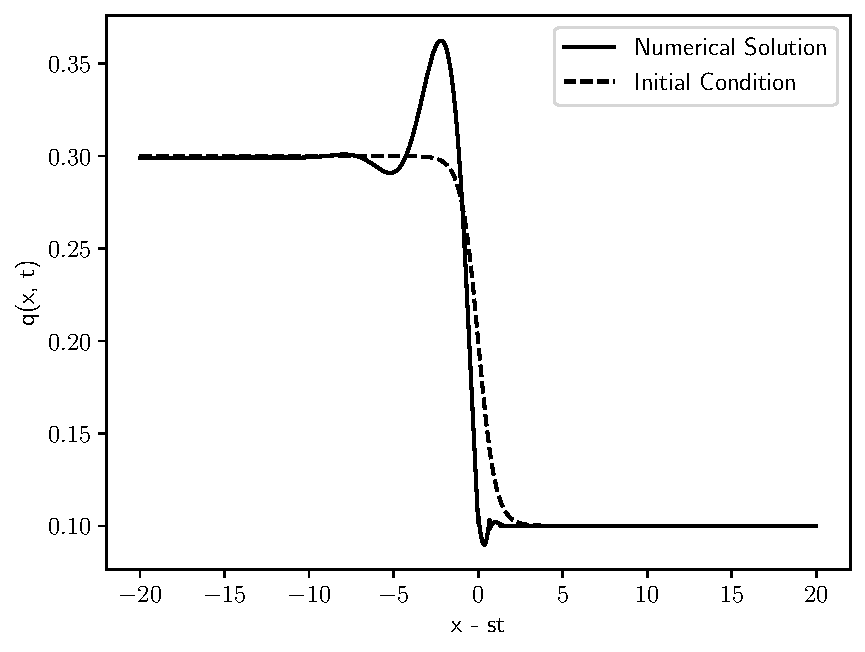
\includegraphics[scale=0.4]{Figures/case_1_1.pdf}
        \end{center}
      \end{frame}

      \begin{frame}
        \frametitle{Wave Structure with Nonlinear Hyper Diffusion}
        \[
          q_r = 0.1 \qquad q_l = 0.3323
        \]
        \[
          q(x, 0) = \p{-\tanh{x} + 1}\frac{q_l - q_r}{2} + q_r
        \]
        \begin{center}
          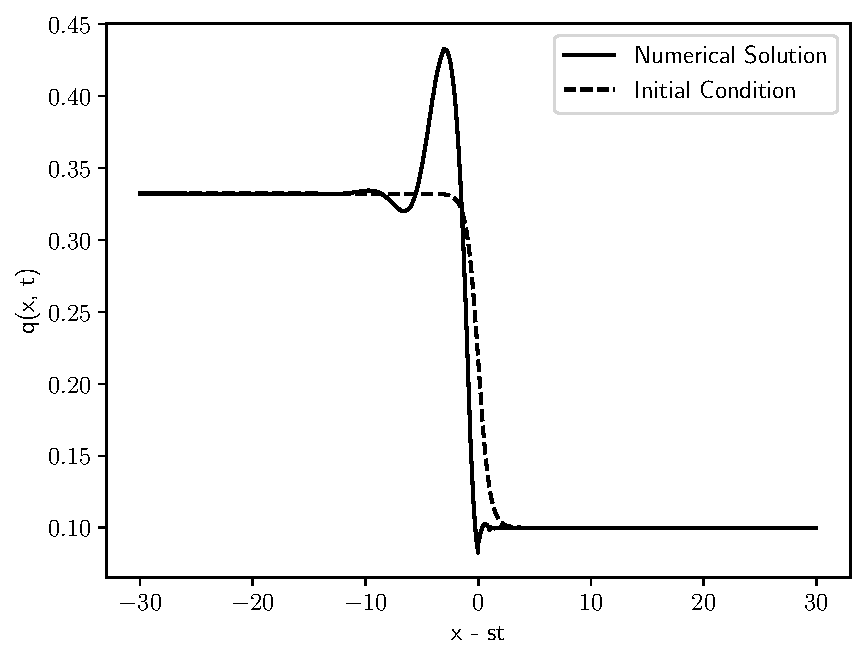
\includegraphics[scale=0.4]{Figures/case_2_1.pdf}
        \end{center}
      \end{frame}

      \begin{frame}
        \frametitle{Wave Structure with Nonlinear Hyper Diffusion}
        \[
          q_r = 0.1 \qquad q_l = 0.3323 \qquad q_m = 0.6
        \]
        \[
          q(x, 0) =
          \begin{cases}
            \frac{q_m - q_l}{2}\tanh{x} + \frac{q_m + q_l}{2} & x < 5 \\
            -\frac{q_m - q_r}{2}\tanh{x - 10} + \frac{q_m + q_r}{2} + q_r & x > 5 \\
          \end{cases}
        \]
        \begin{center}
          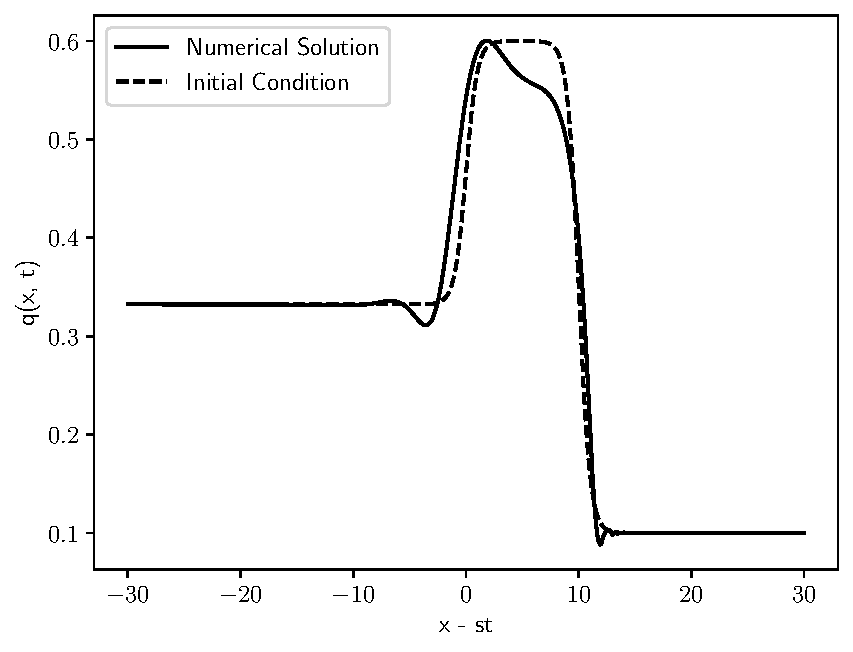
\includegraphics[scale=0.4]{Figures/case_2_2.pdf}
        \end{center}
      \end{frame}

      \begin{frame}
        \frametitle{Wave Structure with Nonlinear Hyper Diffusion}
        \[
          q_r = 0.1 \qquad q_l = 0.3323 \qquad q_m = 0.6
        \]
        \[
          q(x, 0) =
          \begin{cases}
            \frac{q_m - q_l}{2}\tanh{x} + \frac{q_m + q_l}{2} & x < 10 \\
            -\frac{q_m - q_r}{2}\tanh{x - 20} + \frac{q_m + q_r}{2} + q_r & x > 10 \\
          \end{cases}
        \]
        \begin{center}
          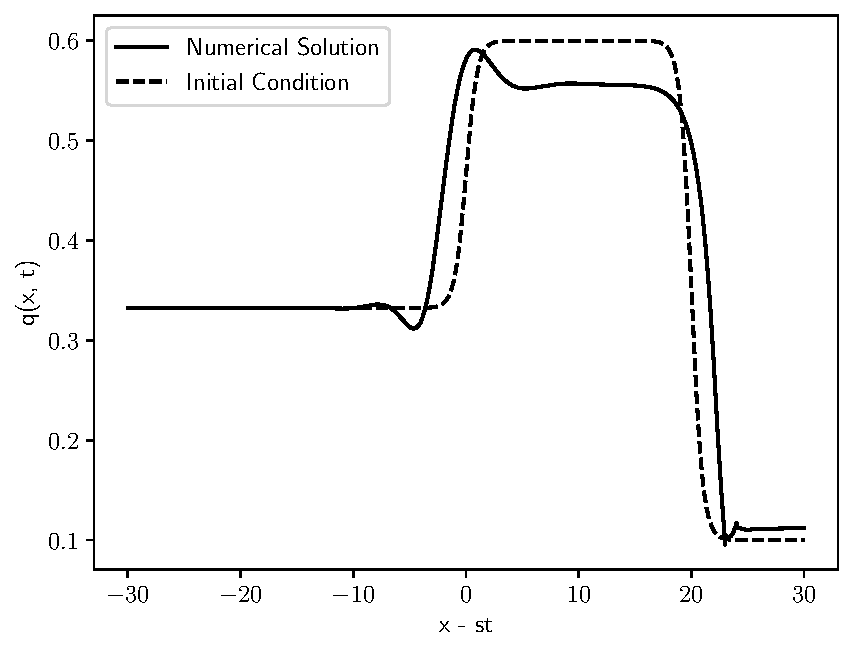
\includegraphics[scale=0.4]{Figures/case_2_3.pdf}
        \end{center}
      \end{frame}

      \begin{frame}
        \frametitle{Wave Structure with Nonlinear Hyper Diffusion}
        \[
          q_r = 0.1 \qquad q_l = 0.4
        \]
        \[
          q(x, 0) = \p{-\tanh{x - 100} + 1}\frac{q_l - q_r}{2} + q_r
        \]
        \begin{center}
          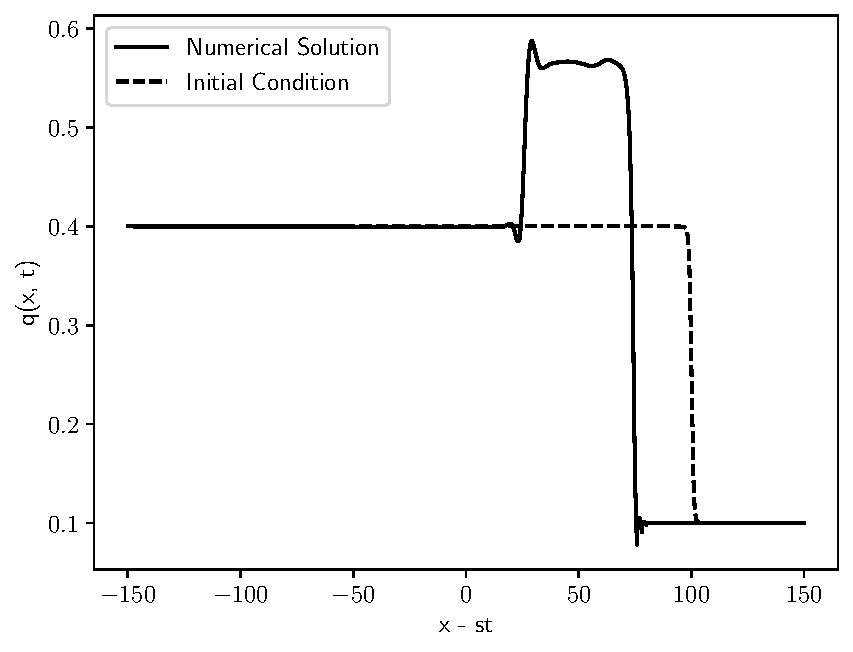
\includegraphics[scale=0.4]{Figures/case_3_1.pdf}
        \end{center}
      \end{frame}

      \begin{frame}
        \frametitle{Wave Structure with Nonlinear Hyper Diffusion}
        \[
          q_r = 0.1 \qquad q_l = 0.8
        \]
        \[
          q(x, 0) = \p{-\tanh{x - 10} + 1}\frac{q_l - q_r}{2} + q_r
        \]
        \begin{center}
          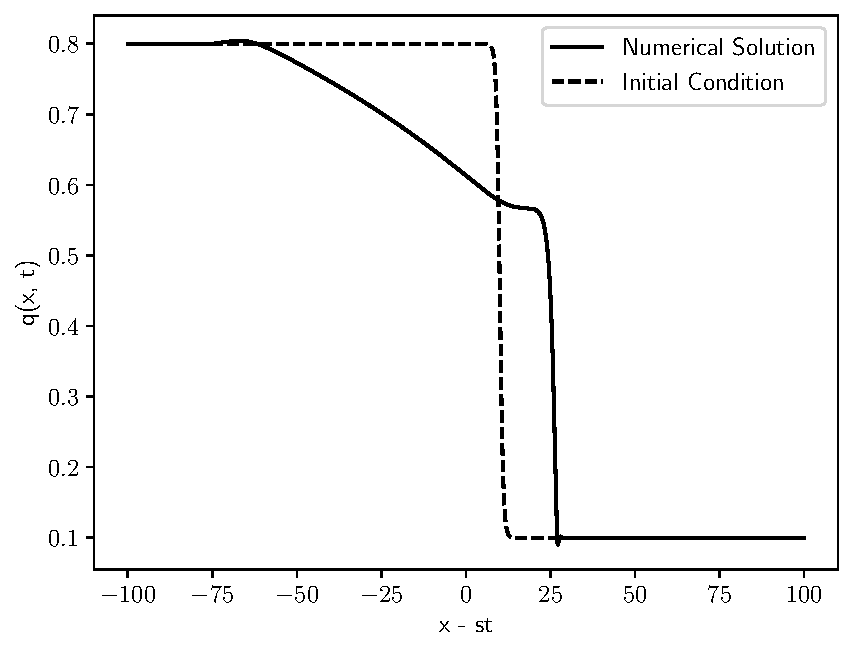
\includegraphics[scale=0.4]{Figures/case_4_1.pdf}
        \end{center}
      \end{frame}

  \section{Generalized Shallow Water Equations}
    \subsection{Model}
      \begin{frame}
        \frametitle{Nondimensionalization}

      \end{frame}

      \begin{frame}
        \frametitle{Mapping}

      \end{frame}

      \begin{frame}
        \frametitle{Newton Closure}

      \end{frame}

    \subsection{Numerical Methods}
      \begin{frame}
        \frametitle{Nonconservative Flux}

        \begin{gather*}
          \dintt{}{}{Q \v{q}_x \phi}{x}
        \end{gather*}

        \begin{gather*}
          \begin{bmatrix}
            Q_x^1 \\
            Q_x^2 \\
            Q_x^3 \\
            Q_x^4 \\
            Q_x^5
          \end{bmatrix}
          = \frac{1}{2\Delta x}
          \begin{bmatrix}
            \Delta Q^1 - 2\sqrt{5} \Delta Q^3 + 78 \Delta Q^5 \\
            \Delta Q^2 - \frac{10}{3} \sqrt{3} \sqrt{7} \Delta Q^4 \\
            \Delta Q^3 - 14 \sqrt{5} \Delta Q^5 \\
            \Delta Q^4 \\
            \Delta Q^5
          \end{bmatrix}
        \end{gather*}

      \end{frame}

    \subsection{Results}
      

    \subsection{Future Work}
      % higher moments
      % two dimension
      % icosahedral mesh
      % slope limiters
      % positivity preserving limiters

    \begin{frame}[allowframebreaks]
      \frametitle{Bibliography}
      % TODO: Bibliography
      \nocite{*}
      \printbibliography{}
    \end{frame}

\end{document}
